\documentclass[man,floatsintext]{apa6}
\usepackage{lmodern}
\usepackage{amssymb,amsmath}
\usepackage{ifxetex,ifluatex}
\usepackage{fixltx2e} % provides \textsubscript
\ifnum 0\ifxetex 1\fi\ifluatex 1\fi=0 % if pdftex
  \usepackage[T1]{fontenc}
  \usepackage[utf8]{inputenc}
\else % if luatex or xelatex
  \ifxetex
    \usepackage{mathspec}
  \else
    \usepackage{fontspec}
  \fi
  \defaultfontfeatures{Ligatures=TeX,Scale=MatchLowercase}
\fi
% use upquote if available, for straight quotes in verbatim environments
\IfFileExists{upquote.sty}{\usepackage{upquote}}{}
% use microtype if available
\IfFileExists{microtype.sty}{%
\usepackage{microtype}
\UseMicrotypeSet[protrusion]{basicmath} % disable protrusion for tt fonts
}{}
\usepackage{hyperref}
\hypersetup{unicode=true,
            pdftitle={Understanding mixed effects models through simulating data},
            pdfauthor={Lisa M. DeBruine~\& Dale J. Barr},
            pdfkeywords={simulation, mixed effect models, power, lme4},
            pdfborder={0 0 0},
            breaklinks=true}
\urlstyle{same}  % don't use monospace font for urls
\usepackage{color}
\usepackage{fancyvrb}
\newcommand{\VerbBar}{|}
\newcommand{\VERB}{\Verb[commandchars=\\\{\}]}
\DefineVerbatimEnvironment{Highlighting}{Verbatim}{commandchars=\\\{\}}
% Add ',fontsize=\small' for more characters per line
\usepackage{framed}
\definecolor{shadecolor}{RGB}{248,248,248}
\newenvironment{Shaded}{\begin{snugshade}}{\end{snugshade}}
\newcommand{\KeywordTok}[1]{\textcolor[rgb]{0.13,0.29,0.53}{\textbf{#1}}}
\newcommand{\DataTypeTok}[1]{\textcolor[rgb]{0.13,0.29,0.53}{#1}}
\newcommand{\DecValTok}[1]{\textcolor[rgb]{0.00,0.00,0.81}{#1}}
\newcommand{\BaseNTok}[1]{\textcolor[rgb]{0.00,0.00,0.81}{#1}}
\newcommand{\FloatTok}[1]{\textcolor[rgb]{0.00,0.00,0.81}{#1}}
\newcommand{\ConstantTok}[1]{\textcolor[rgb]{0.00,0.00,0.00}{#1}}
\newcommand{\CharTok}[1]{\textcolor[rgb]{0.31,0.60,0.02}{#1}}
\newcommand{\SpecialCharTok}[1]{\textcolor[rgb]{0.00,0.00,0.00}{#1}}
\newcommand{\StringTok}[1]{\textcolor[rgb]{0.31,0.60,0.02}{#1}}
\newcommand{\VerbatimStringTok}[1]{\textcolor[rgb]{0.31,0.60,0.02}{#1}}
\newcommand{\SpecialStringTok}[1]{\textcolor[rgb]{0.31,0.60,0.02}{#1}}
\newcommand{\ImportTok}[1]{#1}
\newcommand{\CommentTok}[1]{\textcolor[rgb]{0.56,0.35,0.01}{\textit{#1}}}
\newcommand{\DocumentationTok}[1]{\textcolor[rgb]{0.56,0.35,0.01}{\textbf{\textit{#1}}}}
\newcommand{\AnnotationTok}[1]{\textcolor[rgb]{0.56,0.35,0.01}{\textbf{\textit{#1}}}}
\newcommand{\CommentVarTok}[1]{\textcolor[rgb]{0.56,0.35,0.01}{\textbf{\textit{#1}}}}
\newcommand{\OtherTok}[1]{\textcolor[rgb]{0.56,0.35,0.01}{#1}}
\newcommand{\FunctionTok}[1]{\textcolor[rgb]{0.00,0.00,0.00}{#1}}
\newcommand{\VariableTok}[1]{\textcolor[rgb]{0.00,0.00,0.00}{#1}}
\newcommand{\ControlFlowTok}[1]{\textcolor[rgb]{0.13,0.29,0.53}{\textbf{#1}}}
\newcommand{\OperatorTok}[1]{\textcolor[rgb]{0.81,0.36,0.00}{\textbf{#1}}}
\newcommand{\BuiltInTok}[1]{#1}
\newcommand{\ExtensionTok}[1]{#1}
\newcommand{\PreprocessorTok}[1]{\textcolor[rgb]{0.56,0.35,0.01}{\textit{#1}}}
\newcommand{\AttributeTok}[1]{\textcolor[rgb]{0.77,0.63,0.00}{#1}}
\newcommand{\RegionMarkerTok}[1]{#1}
\newcommand{\InformationTok}[1]{\textcolor[rgb]{0.56,0.35,0.01}{\textbf{\textit{#1}}}}
\newcommand{\WarningTok}[1]{\textcolor[rgb]{0.56,0.35,0.01}{\textbf{\textit{#1}}}}
\newcommand{\AlertTok}[1]{\textcolor[rgb]{0.94,0.16,0.16}{#1}}
\newcommand{\ErrorTok}[1]{\textcolor[rgb]{0.64,0.00,0.00}{\textbf{#1}}}
\newcommand{\NormalTok}[1]{#1}
\usepackage{longtable,booktabs}
\usepackage{graphicx,grffile}
\makeatletter
\def\maxwidth{\ifdim\Gin@nat@width>\linewidth\linewidth\else\Gin@nat@width\fi}
\def\maxheight{\ifdim\Gin@nat@height>\textheight\textheight\else\Gin@nat@height\fi}
\makeatother
% Scale images if necessary, so that they will not overflow the page
% margins by default, and it is still possible to overwrite the defaults
% using explicit options in \includegraphics[width, height, ...]{}
\setkeys{Gin}{width=\maxwidth,height=\maxheight,keepaspectratio}
\IfFileExists{parskip.sty}{%
\usepackage{parskip}
}{% else
\setlength{\parindent}{0pt}
\setlength{\parskip}{6pt plus 2pt minus 1pt}
}
\setlength{\emergencystretch}{3em}  % prevent overfull lines
\providecommand{\tightlist}{%
  \setlength{\itemsep}{0pt}\setlength{\parskip}{0pt}}
\setcounter{secnumdepth}{0}
% Redefines (sub)paragraphs to behave more like sections
\ifx\paragraph\undefined\else
\let\oldparagraph\paragraph
\renewcommand{\paragraph}[1]{\oldparagraph{#1}\mbox{}}
\fi
\ifx\subparagraph\undefined\else
\let\oldsubparagraph\subparagraph
\renewcommand{\subparagraph}[1]{\oldsubparagraph{#1}\mbox{}}
\fi

%%% Use protect on footnotes to avoid problems with footnotes in titles
\let\rmarkdownfootnote\footnote%
\def\footnote{\protect\rmarkdownfootnote}


  \title{Understanding mixed effects models through simulating data}
    \author{Lisa M. DeBruine\textsuperscript{1}~\& Dale J. Barr\textsuperscript{1}}
    \date{}
  
\shorttitle{Simulating for LMEM}
\affiliation{
\vspace{0.5cm}
\textsuperscript{1} Institute of Neuroscience and Psychology, University of Glasgow}
\keywords{simulation, mixed effect models, power, lme4\newline\indent Word count: X}
\usepackage{csquotes}
\usepackage{upgreek}
\captionsetup{font=singlespacing,justification=justified}

\usepackage{longtable}
\usepackage{lscape}
\usepackage{multirow}
\usepackage{tabularx}
\usepackage[flushleft]{threeparttable}
\usepackage{threeparttablex}

\newenvironment{lltable}{\begin{landscape}\begin{center}\begin{ThreePartTable}}{\end{ThreePartTable}\end{center}\end{landscape}}

\makeatletter
\newcommand\LastLTentrywidth{1em}
\newlength\longtablewidth
\setlength{\longtablewidth}{1in}
\newcommand{\getlongtablewidth}{\begingroup \ifcsname LT@\roman{LT@tables}\endcsname \global\longtablewidth=0pt \renewcommand{\LT@entry}[2]{\global\advance\longtablewidth by ##2\relax\gdef\LastLTentrywidth{##2}}\@nameuse{LT@\roman{LT@tables}} \fi \endgroup}


\usepackage{lineno}

\linenumbers

\authornote{

Correspondence concerning this article should be addressed to Lisa M.
DeBruine, 62 Hillhead Street, Glasgow, G12 8QB. E-mail:
\href{mailto:lisa.debruine@glasgow.ac.uk}{\nolinkurl{lisa.debruine@glasgow.ac.uk}}}

\abstract{
Experimental designs that sample both subjects and stimuli from a larger
population need to account for random effects of both subjects and
stimuli using mixed effects models. However, much of this research is
analyzed using ANOVA on aggregated responses because researchers are not
confident specifying and interpreting mixed effects models. The tutorial
will explain how to simulate data with random effects structure and
analyse the data using linear mixed effects regression (with the lme4 R
package). The focus will be on interpreting the LMER output in light of
the simulated parameters, using this method for power calculations, and
comparing the results to by-items and by-subjects ANOVA.


}

\begin{document}
\maketitle

\subsection{Generalizing to a population of
encounters}\label{generalizing-to-a-population-of-encounters}

Many research questions in psychology and neuroscience are questions
about certain types of \emph{events}: What happens when people encounter
particular types of stimuli? For example: Do people recognize abstract
words faster than concrete words? What impressions do people form about
a target person's personality based on their vocal qualities? Can people
categorize emotional expressions more quickly on the faces of social
in-group members than on the faces of out-group members? How do brains
respond to threatening versus non-threatening stimuli? In all of these
situations, researchers would like to be able to make general statements
about phenomena that go beyond the particular participants and
particular stimuli that they happen to have chosen for the specific
study. Traditionally, people speak of such designs as having
\emph{crossed random factors} of participants and stimuli, and have
discussed the problem as one of simultaneous generalization to both
populations. However, it may be more intuitive to think of the problem
as wanting to generalize to a single population of events: in
particular, to a population of \emph{encounters} between the units from
the sampled populations (Barr, 2018).

Most analyses using conventional statistical techniques, such as
analysis of variance and t-test, commit the fallacy of treating stimuli
as fixed rather than random. The problem, and the solutions to the
problem, have been known in psycholinguistics for over 50 years
(Coleman, 1964,Clark (1973)), and most psycholinguistic journals require
authors to demonstrate generality of findings over stimuli as well as
over subjects. Even so, the quasi-\(F\) statistics for ANOVA (\(F'\) and
min-\(F'\)) that Clark proposed as a solution were widely recognized as
unreasonably conservative (Forster \& Dickinson, 1976), and until fairly
recently, most psycholinguists performed separate by-subjects (\(F_1\))
and by-items analyses (\(F_2\)), declaring an effect
\enquote{significant} only if it was significant for both analyses. The
\(F_1 \times F_2\) approach was widely used, despite the fact that Clark
had already shown it to be invalid, since both \(F\) statistics have
higher than nominal false positives in the presence of a null effect,
\(F_1\) due to unmodeled stimulus variance, and \(F_2\) due to unmodeled
subject variance.

Recently, psycholinguists have adopted linear mixed-effects modeling as
the standard for the statistical analysis, given numerous advantages
over ANOVA, including the ability to simultaneously model subject and
stimulus variation, to gracefully deal with missing data or unbalanced
designs, and to accommodate arbitrary types of continuous and
categorical predictors or response variables (Baayen, Davidson, \&
Bates, 2008,Locker, Hoffman, and Bovaird (2007)). This development has
been facilitated by the \texttt{lme4} package for R (D. Bates, Mächler,
Bolker, \& Walker, 2015), which provides powerful functionality for
model specification and estimation. With an appropriately specified
model, mixed-effects models yield major improvements in power over
quasi-\(F\) approaches and avoid the increased false positive rate
associated with separate \(F_1\) and \(F_2\) (Barr, Levy, Scheepers, \&
Tily, 2013).

Despite mixed-effects modeling becoming the \emph{de facto} standard for
analysis in psycholinguistics, the approach has yet to take hold in
other areas where stimuli are routinely sampled, even in spite of
repeated calls for improved analyses in social psychology (Judd,
Westfall, \& Kenny, 2012) and neuroimaging (Bedny, Aguirre, \&
Thompson-Schill, 2007,Westfall, Nichols, and Yarkoni (2016)). One of the
likely reasons for the limited uptake outside of psycholinguistics is
because mixed-effects models expose the analyst to a level of
statistical and technical complexity far beyond most researchers'
training. While some of this complexity is specific to mixed-effects
modeling, some of it is simply hidden away from users of traditional
techniques by GUIs and function defaults. The novice mixed modeler is
suddenly confronted with the need to make decisions about how to specify
categorical predictors, which random effects to include or exclude,
which of the statistics in the voluminous output to attend to, and
whether and how to re-configure the optimizer function when a
convergence error or singularity warning appears.

We are optimisic that the increasing adoption of the mixed-effects
approach will improve the generality and thus reproducibility of studies
in psychology and related fields, but empathize with the frustration ---
and sometimes, exasperation --- expressed by many novices when they
attempt to grapple with these models in their research. Much of the
uncertainty and unease around mixed-effects models comes from using them
in situations where the ground truth is unknown. A profitable way to
improve understanding and user confidence is through data simulation.
Knowing the ground truth allows the user to experiment with various
modeling choices and observe their impact on a model's performance.

\subsection{Simulating data with crossed random
factors}\label{simulating-data-with-crossed-random-factors}

To give an overview of the simulation task, we will simulate data from a
design with crossed random factors of subjects and stimuli, fit a model
to the simulated data, and then try to recover the parameter values we
put in from the output. In this hypothetical study, subjects classify
the emotional expressions of faces as quickly as possible, and we use
their response time as the primary dependent variable. Let's imagine
that the faces are of two intrinsic types: either from the subject's
in-group or from an out-group. For simplicity, we further assume that
each face appears only once in the stimulus set and expresses only one
of two possible emotions (e.g., happiness or anger). The key question is
whether there is any difference in classification speed across the type
of face.

\subsubsection{Required software}\label{required-software}

The simulation will be presented in the R programming language (R Core
Team, 2018). To run the code, you will need to have some add-on packages
available. Any packages you are missing can be installed using R's
\texttt{install.packages()} function, except for the development package
\texttt{faux} (DeBruine, 2019) which, at the time of writing, must be
installed from the development repository on github.

\begin{Shaded}
\begin{Highlighting}[]
\KeywordTok{library}\NormalTok{(}\StringTok{"lme4"}\NormalTok{)        }\CommentTok{# model specification / estimation}
\KeywordTok{library}\NormalTok{(}\StringTok{"afex"}\NormalTok{)        }\CommentTok{# anova and deriving p-values from lmer}
\KeywordTok{library}\NormalTok{(}\StringTok{"broom.mixed"}\NormalTok{) }\CommentTok{# extracting data from model fits }
\KeywordTok{library}\NormalTok{(}\StringTok{"faux"}\NormalTok{)        }\CommentTok{# data simulation}
\CommentTok{# }\AlertTok{NOTE}\CommentTok{: to install the 'faux' package, use:}
\CommentTok{# devtools::install_github("debruine/faux")}
\KeywordTok{library}\NormalTok{(}\StringTok{"tidyverse"}\NormalTok{)   }\CommentTok{# data wrangling and visualisation}
\end{Highlighting}
\end{Shaded}

Because the code uses random number generation, if you want to reproduce
the exact results below you will need to set the random number seed at
the top of your script and ensure you are using R version 3.6.0 or
higher. If you change the seed or are using a lower version of R, your
exact numbers will differ, but the procedure will still produce a valid
simulation.

\begin{Shaded}
\begin{Highlighting}[]
\KeywordTok{set.seed}\NormalTok{(}\DecValTok{8675309}\NormalTok{)}
\end{Highlighting}
\end{Shaded}

\subsubsection{Establishing the data-generating
parameters}\label{establishing-the-data-generating-parameters}

The first thing to do is to set up the parameters that govern the
process we assume to give rise to the data, the \emph{data-generating
process} or DGP. In this hypothetical study, each of 100 subjects will
respond to all 50 stimulus items (25 in-group and 25 out-group), for a
total of 5000 observations.

\paragraph{Specify the data structure}\label{specify-the-data-structure}

We want the resulting data to be in long format, with the structure
shown below, where each row is a single observation for each trial. The
variables \texttt{subj\_id} run from \texttt{S001} to \texttt{S100} and
index the subject number; \texttt{item\_id} runs from \texttt{I01} to
\texttt{I50} and indexes the item number; \texttt{condition} says
whether the face is in-group or out-group, with items 1-25 always
ingroup and items 26-50 always outgroup; and \texttt{RT} is the
participant's response time for that trial. Note that a trial is
uniquely identified by the combination of the \texttt{subj\_id} and
\texttt{item\_id} labels.

\begin{table}[tbp]
\begin{center}
\begin{threeparttable}
\caption{\label{tab:data-example}The target data structure.}
\begin{tabular}{rlllr}
\toprule
row & \multicolumn{1}{c}{subj\_id} & \multicolumn{1}{c}{item\_id} & \multicolumn{1}{c}{condition} & \multicolumn{1}{c}{RT}\\
\midrule
1 & S001 & I01 & ingroup & 750.2\\
2 & S001 & I02 & ingroup & 836.1\\
... & ... & ... & ... & ...\\
49 & S001 & I49 & outgroup & 811.9\\
50 & S001 & I50 & outgroup & 801.8\\
51 & S002 & I01 & ingroup & 806.7\\
52 & S002 & I02 & ingroup & 805.9\\
... & ... & ... & ... & ...\\
5000 & S100 & I50 & outgroup & 859.9\\
\bottomrule
\end{tabular}
\end{threeparttable}
\end{center}
\end{table}

Note that for independent variables in designs where subjects and
stimuli are crossed, you can't think of factors as being solely
\enquote{within} or \enquote{between} because we have two sampling
units; you must ask not only whether independent variables are within-
or between- subjects, but also whether they are within- or between-
stimulus items. Recall that a within-subjects factor is one where each
and every subject receives all of the levels, and a between-subjects
factors is one where each subject receives only one of the levels.
Likewise, a within-subjects factor is one where each stimulus appears
across all of the levels of the independent factors. For our current
example, this is clearly not the case, given that each stimulus item is
either in-group or out-group.

Let's first define parameters related to the number of observations.

\begin{Shaded}
\begin{Highlighting}[]
\NormalTok{nsubj  <-}\StringTok{ }\DecValTok{100} \CommentTok{# number of subjects}
\NormalTok{nitem  <-}\StringTok{ }\KeywordTok{c}\NormalTok{(}\DataTypeTok{ingroup =} \DecValTok{25}\NormalTok{, }\DataTypeTok{outgroup =} \DecValTok{25}\NormalTok{)  }\CommentTok{# number of items}
\end{Highlighting}
\end{Shaded}

\paragraph{Specify the fixed effects}\label{specify-the-fixed-effects}

Getting an appropriately structured dataset is the easy part. The
difficult part is randomly generating the RT values. For this, we need
to establish an underlying statistical model. Let us start with a basic
model and build up from there. We want a model of RT for subject \(s\)
and item \(i\) that looks something like:

\[RT_{si} = \beta_0 + \beta_1 X_{i} + e_{si}\]

In other words, it is the sum of an intercept term \(\beta_0\), which in
this example is the grand mean reaction time for the population of
stimuli, plus \(\beta_1\), the mean RT difference between in-group and
out-group stimuli, plus random noise \(e_{si}\). To make \(\beta_0\)
equal the grand mean and \(\beta_1\) the mean out-group minus the mean
in-group RT, we will code the \texttt{condition} variable as -.5 for the
in-group condition and +.5 for the out-group condition.

Although this model is incomplete, we can go ahead and choose parameters
for \(\beta_0\) and \(\beta_1\). For this example, we set a grand mean
of 800 ms and a mean difference of 80 ms. You will need to use
disciplinary expertise and/or pilot data to choose these parameters. For
power calculations, consider setting effects to the smallest effect size
of interest (Lakens, Scheel, \& Isager, 2018).

\begin{Shaded}
\begin{Highlighting}[]
\NormalTok{b0 <-}\StringTok{ }\DecValTok{800} \CommentTok{# intercept; i.e., the grand mean}
\NormalTok{b1 <-}\StringTok{  }\DecValTok{80} \CommentTok{# slope; i.e, effect of condition}
\end{Highlighting}
\end{Shaded}

The parameters \(\beta_0\) and \(\beta_1\) are \emph{fixed effects}:
they characterize properties of the population of encounters between
subjects and stimuli. Thus, we assign the mean RT for a
\enquote{typical} subject encountering a \enquote{typical} stimulus to
800 ms, and that responses are typically 80 ms slower for outgroup than
ingroup faces.

\paragraph{Specify the random effects}\label{specify-the-random-effects}

This model is completely unrealistic, however, because it doesn't allow
for any individual differences among subjects or stimuli. Not all
subjects are typical: some will be faster than average, and some slower.
We can characterize the difference from the grand mean for each subject
\(s\) in terms of a \emph{random effect} \(S_{0s}\), where the first
subscript, 0, indicates that the deflection goes with the intercept
term, \(\beta_0\). In other words, we assume each subject to have a
unique \emph{random intercept}. Likewise, it is unrealistic to assume
that it is equally easy to categorize emotional expressions across all
faces in the dataset; some will be easier than others. We incorporate
this assumption by including by-item random intercepts \(I_{0i}\), with
the subscript 0 reminding us that it is a deflection from the
\(\beta_0\) term, and the \(i\) indicating a unique deflection for each
of the 50 faces. Adding these terms to our model yields:

\[RT_{si} = \beta_0 + S_{0s} + I_{0i} + \beta_1 X_i + e_{si}.\]

Now, the actual values for \(S_{0s}\) and \(I_{0i}\) in our sampled
dataset will depend on the luck of the draw, i.e., on which subject and
which stimuli we happened to have sampled from their respective
populations. So to capture that these are \emph{random} rather than
\emph{fixed} factors, we will set parameters that capture the standard
deviation among the random effects and then use these to
\enquote{sample} from the populations. Below we assign the by-subject
offsets a standard deviation of 100 ms (\texttt{sri\_sd}), and the
by-item offsets have a standard deviation of 80 ms (\texttt{iri\_sd}).
We will discuss below how you can estimate these parameters for your own
designs.

\begin{Shaded}
\begin{Highlighting}[]
\NormalTok{sri_sd <-}\StringTok{ }\DecValTok{100} \CommentTok{# by-subject random intercept sd}
\NormalTok{iri_sd <-}\StringTok{  }\DecValTok{80} \CommentTok{# by-item random intercept sd}
\end{Highlighting}
\end{Shaded}

There is still a deficiency in our data-generating model related to
\(\beta_1\), the fixed effect of condition. Currently our model assumes
that each and every subject is exactly 80 ms faster to categorize
emotions on ingroup faces than on outgroup faces. Clearly, this
assumption is totally unrealistic; some participants will be more
sensitive to ingroup/outgroup differences than others. We can capture
this in an analogous way to which we captured variation in the
intercept, namely by including by-subject \emph{random slopes}
\(S_{1s}\).

\[RT_{si} = \beta_0 + S_{0s} + I_{0i} + \left(\beta_1 + S_{1s}\right) X_i + e_{si}.\]

A participant who is, on average, 90 ms faster for ingroup faces would
have a random slope \(S_{1s} = 10\) (90 = 80 + 10); a participant who
goes against the grain and is, for whatever reason, on average 15 ms
faster for \emph{outgroup} faces would have a random slope of
\(S_{1s} = -95\) (-15 = 80 - 95). As we did for the random intercepts,
we characterize the random slopes in terms of their standard deviation
\texttt{srs\_sd}, which we assign to be 40 ms.

But note that we are sampling \emph{two} random effects for each subject
\(s\), a random intercept \(S_{0s}\) and a random slope \(S_{1s}\). It
is possible for these values to be correlated, in which case we should
not sample them independently. For instance, perhaps people who are
faster than average overall (negative random intercept) also show a
smaller than average of the ingroup/outgroup manipulation (negative
random slope) due to allocating less attention to the task. We can
capture this by allowing for a small correlation between the two
factors, \texttt{scor}, which we assign to be .2.

Finally, we need to characterize the trial-level noise in the study (the
\(e_{si}\)s) in terms of their standard deviations. Here we simply
assign this parameter value \texttt{err\_sd} to be twice the size of the
by-subject random intercept SD.

\begin{Shaded}
\begin{Highlighting}[]
\NormalTok{srs_sd <-}\StringTok{  }\DecValTok{40} \CommentTok{# by-subject random slope sd}
\NormalTok{scor   <-}\StringTok{  }\NormalTok{.}\DecValTok{2} \CommentTok{# correlation between intercept and slope}
\NormalTok{err_sd <-}\StringTok{ }\DecValTok{200} \CommentTok{# residual (error) sd}
\end{Highlighting}
\end{Shaded}

To summarize, we established a reasonable statistical model underlying
the data having the form:

\[RT_{si} = \beta_0 + S_{0s} + I_{0i} + \left(\beta_1 + S_{1s}\right) X_i + e_{si}\]

where the response time for subject \(s\) on item \(i\), \(RT_{si}\), is
decomposed into a population grand mean \(\beta_0\), a by-subject random
intercept \(S_{0s}\), a by-item random intercept \(I_{0i}\), a fixed
slope \(\beta_1\), a by-subject random slope \(S_{1s}\), and a
trial-level residual \(e_{si}\). Our data-generating process is fully
determined by seven parameters: two fixed effects (intercept and slope),
four variance parameters governing the random effects (defined in the
code as \texttt{sri\_sd}, \texttt{srs\_sd}, \texttt{scor}, and
\texttt{iri\_sd}), and one parameter governing the trial level variance
(\texttt{err\_sd}).

In the next section we will apply this data-generating process to
simulate the sampling of subjects, items, and trials (encounters).

\subsubsection{Simulating the sampling
process}\label{simulating-the-sampling-process}

\paragraph{Simulate the sampling of stimulus
items}\label{simulate-the-sampling-of-stimulus-items}

We need to create a table listing each item, which condition it is in,
and simulated values for its random effects. We can do this with the
code below, setting item ID to the numbers 1 through the total number of
items, condition for the first 25 items to \enquote{ingroup} and the
next 25 faces to \enquote{outgroup}, and sampling 50 numbers from a
normal distribution with a mean of 0 and a standard deviation of
\texttt{iri\_sd}.

\begin{Shaded}
\begin{Highlighting}[]
\NormalTok{items <-}\StringTok{ }\KeywordTok{data.frame}\NormalTok{(}
  \DataTypeTok{item_id =} \DecValTok{1}\OperatorTok{:}\KeywordTok{sum}\NormalTok{(nitem),}
  \DataTypeTok{condition =} \KeywordTok{rep}\NormalTok{(}\KeywordTok{c}\NormalTok{(}\StringTok{"ingroup"}\NormalTok{, }\StringTok{"outgroup"}\NormalTok{), nitem),}
  \DataTypeTok{I0i =} \KeywordTok{rnorm}\NormalTok{(}\KeywordTok{sum}\NormalTok{(nitem), }\DecValTok{0}\NormalTok{, iri_sd)}
\NormalTok{)}
\end{Highlighting}
\end{Shaded}

The function \texttt{faux::sim\_design()} is a more flexible way to
generate data with specified parameters. This function will create a
dataset with any number of between and/or within factors, \texttt{n}
items per between-cell, and the specified means (\texttt{mu}), standard
deviations (\texttt{sd}) and correlations (r). By default, it plots a
schematic of the design you specified. See the vignette (DeBruine, 2019)
for more details.

Condition is a between-items factor, so we need to include it in the
\texttt{between} argument. Set \texttt{n\ =\ nitem} to specify the
number of items per condition. Set \texttt{sd\ =\ iri\_sd} to set the
standard deviation for the by-item random effects. Set
\texttt{dv\ =\ "I0i"} to give the random effect column that name. Set
\texttt{id\ =\ "item\_id"}; we'll use this later to join this
information to the table of trials.

\begin{Shaded}
\begin{Highlighting}[]
\NormalTok{items <-}\StringTok{ }\NormalTok{faux}\OperatorTok{::}\KeywordTok{sim_design}\NormalTok{(}
  \DataTypeTok{between =} \KeywordTok{list}\NormalTok{(}\DataTypeTok{condition =} \KeywordTok{c}\NormalTok{(}\StringTok{"ingroup"}\NormalTok{, }\StringTok{"outgroup"}\NormalTok{)),}
  \DataTypeTok{n =}\NormalTok{ nitem,}
  \DataTypeTok{sd =}\NormalTok{ iri_sd,}
  \DataTypeTok{dv =} \StringTok{"I0i"}\NormalTok{,}
  \DataTypeTok{id =} \StringTok{"item_id"}
\NormalTok{)}
\end{Highlighting}
\end{Shaded}

\begin{figure}

{\centering 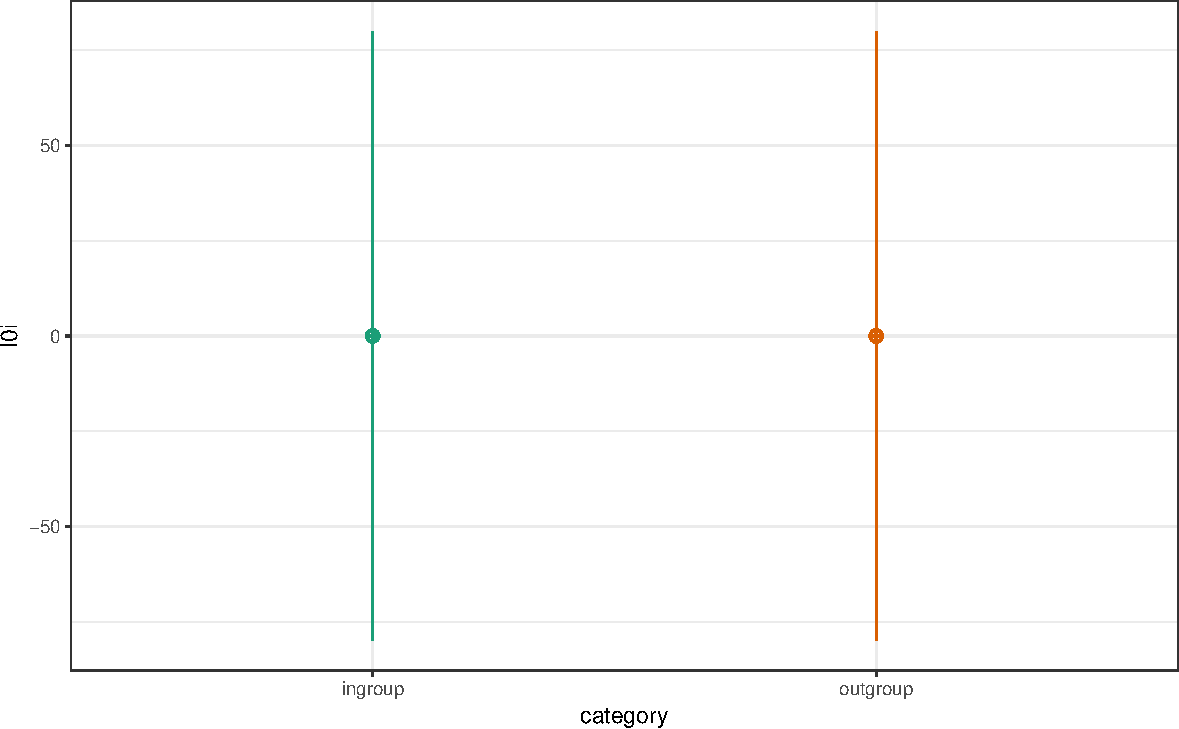
\includegraphics[width=0.75\linewidth]{images/sim-items-1} 

}

\caption{The specified distribution of random effects for ingroup and outgroup faces.}\label{fig:sim-items}
\end{figure}

We will also introduce a numerical predictor to represent what condition
each stimulus item \(i\) appears in (i.e., for the \(X_i\) in our
model). Since we predict that responses to ingroup faces will be faster
than outgroup faces, we set ingroup to -0.5 and outgroup to +0.5. We
will later multiply this \emph{effect coded} factor by the fixed effect
of condition (\texttt{b1} = 80) to simulate data where the ingroup faces
are on average -40 ms different from the grand mean, while the outgroup
faces are 40 ms different from the grand mean.

\begin{Shaded}
\begin{Highlighting}[]
\CommentTok{# effect code condition}
\NormalTok{items}\OperatorTok{$}\NormalTok{cond <-}\StringTok{ }\KeywordTok{recode}\NormalTok{(items}\OperatorTok{$}\NormalTok{condition, }\StringTok{"ingroup"}\NormalTok{ =}\StringTok{ }\OperatorTok{-}\FloatTok{0.5}\NormalTok{, }\StringTok{"outgroup"}\NormalTok{ =}\StringTok{ }\OperatorTok{+}\FloatTok{0.5}\NormalTok{)}
\end{Highlighting}
\end{Shaded}

\begin{table}[tbp]
\begin{center}
\begin{threeparttable}
\caption{\label{tab:items-table}The resulting table of item parameters.}
\begin{tabular}{llll}
\toprule
item\_id & \multicolumn{1}{c}{condition} & \multicolumn{1}{c}{I0i} & \multicolumn{1}{c}{cond}\\
\midrule
S01 & ingroup & 59.56 & -0.50\\
S02 & ingroup & -107.73 & -0.50\\
S03 & ingroup & 26.41 & -0.50\\
S04 & ingroup & -1.02 & -0.50\\
S05 & ingroup & -37.09 & -0.50\\
S06 & ingroup & 16.40 & -0.50\\
\bottomrule
\end{tabular}
\end{threeparttable}
\end{center}
\end{table}

\paragraph{Simulate the sampling of
subjects}\label{simulate-the-sampling-of-subjects}

Now we will simulate the sampling of individual subjects, resulting in a
table listing each subject and their two correlated random effects. We
will again use \texttt{faux::sim\_design()} for this task.

Set the \texttt{within} argument in \texttt{sim\_design()} to a list
with one factor (\texttt{effect}) that has two levels: \texttt{S0s} and
\texttt{S1s}. If you set a factor's levels as a named vector, the names
(\texttt{S0s} and \texttt{S1s}) become the column names in the data
table and the values are used in plots created by faux.

Set \texttt{n\ =\ nsubj} to specify the number of subjects. There are
two random effects to specify standard deviation for, so set \texttt{sd}
using a named vector and set their correlation with r = scor. Set
\texttt{dv\ =\ "value"}; this will only be used in faux plots. Set
\texttt{id\ =\ "subj\_id"}; we'll use this later to join this
information to the table of trials.

\begin{Shaded}
\begin{Highlighting}[]
\NormalTok{subjects <-}\StringTok{ }\NormalTok{faux}\OperatorTok{::}\KeywordTok{sim_design}\NormalTok{(}
  \DataTypeTok{within =} \KeywordTok{list}\NormalTok{(}\DataTypeTok{effect =} \KeywordTok{c}\NormalTok{(}\DataTypeTok{S0s =} \StringTok{"By-subject random intercepts"}\NormalTok{, }
                           \DataTypeTok{S1s =} \StringTok{"By-subject random slopes"}\NormalTok{)), }
  \DataTypeTok{n =}\NormalTok{ nsubj,}
  \DataTypeTok{sd =} \KeywordTok{c}\NormalTok{(}\DataTypeTok{sri_sd =}\NormalTok{ sri_sd, }\DataTypeTok{srs_sd =}\NormalTok{ srs_sd), }
  \DataTypeTok{r =}\NormalTok{ scor,}
  \DataTypeTok{dv =} \StringTok{"value"}\NormalTok{,}
  \DataTypeTok{id =} \StringTok{"subj_id"}
\NormalTok{)}
\end{Highlighting}
\end{Shaded}

\begin{figure}

{\centering 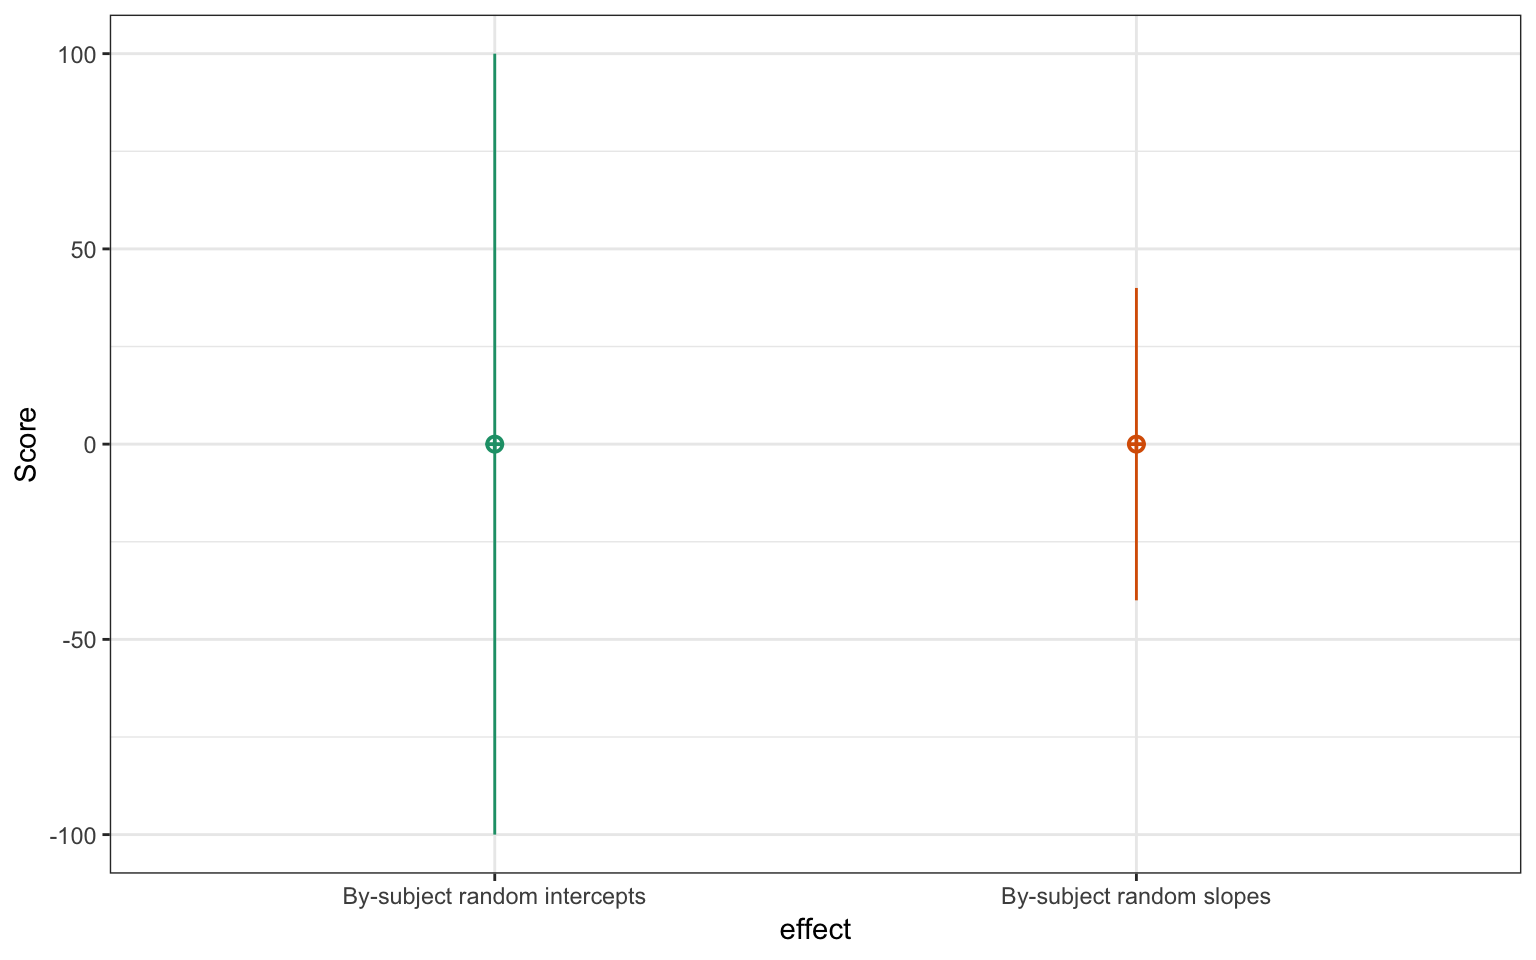
\includegraphics[width=0.75\linewidth]{images/sim-subjects-1} 

}

\caption{The specified distribution of random effects for subjects}\label{fig:sim-subjects}
\end{figure}

Let's have a look at the resulting table.

\begin{table}[tbp]
\begin{center}
\begin{threeparttable}
\caption{\label{tab:subj-table}The resulting table of subject parameters.}
\begin{tabular}{lll}
\toprule
subj\_id & \multicolumn{1}{c}{S0s} & \multicolumn{1}{c}{S1s}\\
\midrule
S001 & -98.77 & -49.49\\
S002 & 37.33 & 23.77\\
S003 & -127.42 & 39.56\\
S004 & -56.37 & 10.13\\
S005 & -39.73 & -8.05\\
S006 & 43.70 & 37.66\\
\bottomrule
\end{tabular}
\end{threeparttable}
\end{center}
\end{table}

\paragraph{Simulate trials
(encounters)}\label{simulate-trials-encounters}

Since all subjects respond to all items, we can set up a table of trials
by crossing the subject IDs with the item IDs. Each trial has random
error associated; we simulate this from a normal distribution with a
mean of 0 and SD of \texttt{err\_sd}.

\begin{Shaded}
\begin{Highlighting}[]
\CommentTok{# crossing() is from the tidyr package; }
\CommentTok{# see ?tidyr::crossing for details}
\NormalTok{trials <-}\StringTok{ }\KeywordTok{crossing}\NormalTok{(}\DataTypeTok{subj_id =}\NormalTok{ subjects}\OperatorTok{$}\NormalTok{subj_id,}
                   \DataTypeTok{item_id =}\NormalTok{ items}\OperatorTok{$}\NormalTok{item_id) }\OperatorTok
\StringTok{  }\KeywordTok{mutate}\NormalTok{(}\DataTypeTok{err =} \KeywordTok{rnorm}\NormalTok{(}\KeywordTok{nrow}\NormalTok{(.), }\DataTypeTok{mean =} \DecValTok{0}\NormalTok{, }\DataTypeTok{sd =}\NormalTok{ err_sd))}
\end{Highlighting}
\end{Shaded}

\begin{table}[tbp]
\begin{center}
\begin{threeparttable}
\caption{\label{tab:trials-table}The resulting table of trials.}
\begin{tabular}{lll}
\toprule
subj\_id & \multicolumn{1}{c}{item\_id} & \multicolumn{1}{c}{err}\\
\midrule
S001 & S01 & 307.99\\
S001 & S02 & 85.33\\
S001 & S03 & -205.25\\
S001 & S04 & -138.06\\
S001 & S05 & -190.78\\
S001 & S06 & -351.12\\
\bottomrule
\end{tabular}
\end{threeparttable}
\end{center}
\end{table}

\subsubsection{Calculate the response
values}\label{calculate-the-response-values}

Now that we have a table of all trials, we can join the information in
this table to the information in our \texttt{subjects} and
\texttt{items} tables. We join them together using
\texttt{dplyr::inner\_join()}.

\begin{Shaded}
\begin{Highlighting}[]
\NormalTok{joined <-}\StringTok{ }\NormalTok{trials }\OperatorTok
\StringTok{  }\KeywordTok{inner_join}\NormalTok{(subjects, }\StringTok{"subj_id"}\NormalTok{) }\OperatorTok
\StringTok{  }\KeywordTok{inner_join}\NormalTok{(items, }\StringTok{"item_id"}\NormalTok{)}
\end{Highlighting}
\end{Shaded}

\begin{table}[tbp]
\begin{center}
\begin{threeparttable}
\caption{\label{tab:joined-table}The resulting table of trials joined to subject and item parameters.}
\begin{tabular}{llllllll}
\toprule
subj\_id & \multicolumn{1}{c}{item\_id} & \multicolumn{1}{c}{err} & \multicolumn{1}{c}{S0s} & \multicolumn{1}{c}{S1s} & \multicolumn{1}{c}{condition} & \multicolumn{1}{c}{I0i} & \multicolumn{1}{c}{cond}\\
\midrule
S001 & S01 & 307.99 & -98.77 & -49.49 & ingroup & 59.56 & -0.50\\
S001 & S02 & 85.33 & -98.77 & -49.49 & ingroup & -107.73 & -0.50\\
S001 & S03 & -205.25 & -98.77 & -49.49 & ingroup & 26.41 & -0.50\\
S001 & S04 & -138.06 & -98.77 & -49.49 & ingroup & -1.02 & -0.50\\
S001 & S05 & -190.78 & -98.77 & -49.49 & ingroup & -37.09 & -0.50\\
S001 & S06 & -351.12 & -98.77 & -49.49 & ingroup & 16.40 & -0.50\\
\bottomrule
\end{tabular}
\end{threeparttable}
\end{center}
\end{table}

Note how this resulting table contains the full decomposition of effects
that we need to compute the response according to the linear model we
defined above:

\[RT_{si} = \beta_0 + S_{0s} + I_{0i} + \left(\beta_1 + S_{1s}\right) X_i + e_{si}.\]

Thus, we will calculate the response variable \texttt{RT} by adding
together:

\begin{itemize}
\tightlist
\item
  the grand intercept (\texttt{b0}),
\item
  each subject-specific random intercept (\texttt{S0s}),
\item
  each item-specific random intercept (\texttt{I0i}),
\item
  each sum of the condition effect (\texttt{b1}) and the random slope
  (\texttt{S1s}), multiplied by the numerical predictor (\texttt{cond}),
  and
\item
  each residual error (\texttt{err}).
\end{itemize}

After this we will use \texttt{dplyr::select()} to keep the columns we
need. Note that the resulting table has the structure that we set as our
goal at the start of this exercise, with the additional column
\texttt{cond} which we will keep around to use in the estimation
process, described in the next section.

\begin{Shaded}
\begin{Highlighting}[]
\NormalTok{dat_sim <-}\StringTok{ }\NormalTok{joined }\OperatorTok
\StringTok{  }\KeywordTok{mutate}\NormalTok{(}\DataTypeTok{RT =}\NormalTok{ b0 }\OperatorTok{+}\StringTok{ }\NormalTok{S0s }\OperatorTok{+}\StringTok{ }\NormalTok{I0i }\OperatorTok{+}\StringTok{ }\NormalTok{(b1 }\OperatorTok{+}\StringTok{ }\NormalTok{S1s) }\OperatorTok{*}\StringTok{ }\NormalTok{cond }\OperatorTok{+}\StringTok{ }\NormalTok{err) }\OperatorTok
\StringTok{  }\KeywordTok{select}\NormalTok{(subj_id, item_id, condition, cond, RT)}
\end{Highlighting}
\end{Shaded}

\begin{table}[tbp]
\begin{center}
\begin{threeparttable}
\caption{\label{tab:dat-sim-table}The final simulated dataset.}
\begin{tabular}{lllll}
\toprule
subj\_id & \multicolumn{1}{c}{item\_id} & \multicolumn{1}{c}{condition} & \multicolumn{1}{c}{cond} & \multicolumn{1}{c}{RT}\\
\midrule
S001 & S01 & ingroup & -0.50 & 1,053.53\\
S001 & S02 & ingroup & -0.50 & 663.58\\
S001 & S03 & ingroup & -0.50 & 507.14\\
S001 & S04 & ingroup & -0.50 & 546.90\\
S001 & S05 & ingroup & -0.50 & 458.10\\
S001 & S06 & ingroup & -0.50 & 351.25\\
\bottomrule
\end{tabular}
\end{threeparttable}
\end{center}
\end{table}

\subsection{Analyse Data}\label{analyse-data}

Now we're ready to analyse our simulated data. The formula for
\texttt{lmer()} maps onto how we calculated the response above.

\begin{verbatim}
RT ~ 1 + cond + (1 | item_id) + (1 + cond | subj_id)
\end{verbatim}

\begin{itemize}
\tightlist
\item
  \texttt{RT} is the response
\item
  \texttt{1} is the grand intercept (\texttt{b0}),
\item
  \texttt{cond} is the effect of condition (\texttt{b1\ *\ cond}),
\item
  \texttt{1} in \texttt{(1\ \textbar{}\ item\_id)} is the item-specific
  random intercept (\texttt{iri}),
\item
  \texttt{1} in \texttt{(1\ +\ cond\ \textbar{}\ subj\_id)} is the
  subject-specific random intercept (\texttt{sri}),
\item
  \texttt{cond} in \texttt{(1\ +\ cond\ \textbar{}\ subj\_id)} is the
  subject-specific random slope of condition (\texttt{S1s\ *\ cond})
\end{itemize}

The \texttt{lmer()} function takes this formula as its first argument,
then the data table. Set \texttt{REML\ =\ FALSE} to choose the method
for estimating variance components (\texttt{REML\ =\ TRUE} is better
when you have fairly unequal cell sizes).

\begin{Shaded}
\begin{Highlighting}[]
\NormalTok{mod_sim <-}\StringTok{ }\KeywordTok{lmer}\NormalTok{(RT }\OperatorTok{~}\StringTok{ }\DecValTok{1} \OperatorTok{+}\StringTok{ }\NormalTok{cond }\OperatorTok{+}\StringTok{ }\NormalTok{(}\DecValTok{1} \OperatorTok{|}\StringTok{ }\NormalTok{item_id) }\OperatorTok{+}\StringTok{ }\NormalTok{(}\DecValTok{1} \OperatorTok{+}\StringTok{ }\NormalTok{cond }\OperatorTok{|}\StringTok{ }\NormalTok{subj_id),}
                \DataTypeTok{data =}\NormalTok{ dat_sim, }\DataTypeTok{REML =} \OtherTok{TRUE}\NormalTok{)}
\end{Highlighting}
\end{Shaded}

Use the \texttt{summary()} function to view the results. Notice where
the parameters you set at the beginning show up in the results. If you
analyze existing data with a mixed effect model, you can use these
estimates to help you set reasonable values for random effects in your
own simulations.

\begin{Shaded}
\begin{Highlighting}[]
\KeywordTok{summary}\NormalTok{(mod_sim, }\DataTypeTok{corr =} \OtherTok{FALSE}\NormalTok{)}
\end{Highlighting}
\end{Shaded}

\begin{verbatim}
## Linear mixed model fit by REML. t-tests use Satterthwaite's method [
## lmerModLmerTest]
## Formula: RT ~ 1 + cond + (1 | item_id) + (1 + cond | subj_id)
##    Data: dat_sim
## 
## REML criterion at convergence: 67691.5
## 
## Scaled residuals: 
##     Min      1Q  Median      3Q     Max 
## -3.7638 -0.6737 -0.0046  0.6776  3.6428 
## 
## Random effects:
##  Groups   Name        Variance Std.Dev. Corr
##  subj_id  (Intercept) 10396    101.96       
##           cond         2421     49.21   0.16
##  item_id  (Intercept)  4723     68.72       
##  Residual             40769    201.91       
## Number of obs: 5000, groups:  subj_id, 100; item_id, 50
## 
## Fixed effects:
##             Estimate Std. Error     df t value Pr(>|t|)    
## (Intercept)   816.05      14.37 123.21  56.778  < 2e-16 ***
## cond           82.42      20.85  53.33   3.954 0.000228 ***
## ---
## Signif. codes:  0 '***' 0.001 '**' 0.01 '*' 0.05 '.' 0.1 ' ' 1
\end{verbatim}

\begin{table}[tbp]
\begin{center}
\begin{threeparttable}
\caption{\label{tab:unnamed-chunk-8}The simulation parameters versus the model estimations.}
\begin{tabular}{llll}
\toprule
variable & \multicolumn{1}{c}{explanation} & \multicolumn{1}{c}{simulated value} & \multicolumn{1}{c}{estimated by model}\\
\midrule
b0 & intercept (grand mean) & 800.00 & 816.05\\
b1 & fixed effect of condition & 80.00 & 82.42\\
sri\_sd & by-subject random intercept SD & 100.00 & 101.96\\
srs\_sd & by-subject random slope SD & 40.00 & 49.21\\
scor & cor between intercept and slope & 0.20 & 0.16\\
iri\_sd & by-item random intercept SD & 80.00 & 68.72\\
err\_sd & residual (error) SD & 200.00 & 201.91\\
\bottomrule
\end{tabular}
\end{threeparttable}
\end{center}
\end{table}

You can also use \texttt{broom.mixed::tidy()} to output fixed and/or
random effects in a tidy table. This is especially useful when you need
to combine the output from hundreds of simulations to calculate power.
The code below adds a column with the simulated parameters we set above
so you can compare them to the estimated parameters from this simulated
dataset.

\begin{Shaded}
\begin{Highlighting}[]
\NormalTok{broom.mixed}\OperatorTok{::}\KeywordTok{tidy}\NormalTok{(mod_sim) }\OperatorTok\StringTok{ }
\StringTok{  }\KeywordTok{mutate}\NormalTok{(}\DataTypeTok{sim.params =} \KeywordTok{c}\NormalTok{(b0, b1, sri_sd, srs_sd, scor, iri_sd, err_sd)) }\OperatorTok
\StringTok{  }\KeywordTok{select}\NormalTok{(}\DecValTok{1}\OperatorTok{:}\DecValTok{3}\NormalTok{, }\DecValTok{9}\NormalTok{, }\DecValTok{4}\OperatorTok{:}\DecValTok{8}\NormalTok{) }\OperatorTok
\StringTok{  }\KeywordTok{apa_table}\NormalTok{(}\DataTypeTok{digits =} \DecValTok{3}\NormalTok{, }\DataTypeTok{caption=}\StringTok{"The output of the tidy function from broom.mixed."}\NormalTok{)}
\end{Highlighting}
\end{Shaded}

\begin{table}[tbp]
\begin{center}
\begin{threeparttable}
\caption{\label{tab:unnamed-chunk-9}The output of the tidy function from broom.mixed.}
\begin{tabular}{lllllllll}
\toprule
effect & \multicolumn{1}{c}{group} & \multicolumn{1}{c}{term} & \multicolumn{1}{c}{sim.params} & \multicolumn{1}{c}{estimate} & \multicolumn{1}{c}{std.error} & \multicolumn{1}{c}{statistic} & \multicolumn{1}{c}{df} & \multicolumn{1}{c}{p.value}\\
\midrule
fixed & NA & (Intercept) & 800.000 & 816.045 & 14.373 & 56.778 & 123.214 & 0.000\\
fixed & NA & cond & 80.000 & 82.425 & 20.848 & 3.954 & 53.332 & 0.000\\
ran\_pars & subj\_id & sd\_\_(Intercept) & 100.000 & 101.963 & NA & NA & NA & NA\\
ran\_pars & subj\_id & sd\_\_cond & 40.000 & 49.205 & NA & NA & NA & NA\\
ran\_pars & subj\_id & cor\_\_(Intercept).cond & 0.200 & 0.159 & NA & NA & NA & NA\\
ran\_pars & item\_id & sd\_\_(Intercept) & 80.000 & 68.723 & NA & NA & NA & NA\\
ran\_pars & Residual & sd\_\_Observation & 200.000 & 201.913 & NA & NA & NA & NA\\
\bottomrule
\end{tabular}
\end{threeparttable}
\end{center}
\end{table}

\subsection{Calculate Power}\label{calculate-power}

You can set up a function that takes all of the parameters we set above
as arguments. We'll set the to default to the values we used, but you
can choose your own defaults. The code below is just all of the data
simulation code above, condensed a bit. It returns one dataset with the
parameters you specified.

\begin{Shaded}
\begin{Highlighting}[]
\NormalTok{my_sim_data <-}\StringTok{ }\ControlFlowTok{function}\NormalTok{(}\DataTypeTok{nsubj  =} \DecValTok{100}\NormalTok{, }\CommentTok{# number of subjects}
                        \DataTypeTok{nitem  =} \KeywordTok{c}\NormalTok{(}\DataTypeTok{ingroup =} \DecValTok{25}\NormalTok{, }\DataTypeTok{outgroup =} \DecValTok{25}\NormalTok{),  }\CommentTok{# number of items}
                        \DataTypeTok{b0     =} \DecValTok{800}\NormalTok{, }\CommentTok{# grand mean}
                        \DataTypeTok{b1     =}  \DecValTok{80}\NormalTok{, }\CommentTok{# effect of condition}
                        \DataTypeTok{iri_sd =}  \DecValTok{80}\NormalTok{, }\CommentTok{# by-item random intercept sd}
                        \DataTypeTok{sri_sd =} \DecValTok{100}\NormalTok{, }\CommentTok{# by-subject random intercept sd}
                        \DataTypeTok{srs_sd =}  \DecValTok{40}\NormalTok{, }\CommentTok{# by-subject random slope sd}
                        \DataTypeTok{scor   =} \FloatTok{0.2}\NormalTok{, }\CommentTok{# correlation between intercept and slope}
                        \DataTypeTok{err_sd =} \DecValTok{200}  \CommentTok{# residual (standard deviation)}
\NormalTok{                        ) \{}
  \CommentTok{# simulate items}
\NormalTok{  items <-}\StringTok{ }\NormalTok{faux}\OperatorTok{::}\KeywordTok{sim_design}\NormalTok{(}
    \DataTypeTok{between =} \KeywordTok{list}\NormalTok{(}\DataTypeTok{condition =} \KeywordTok{c}\NormalTok{(}\StringTok{"ingroup"}\NormalTok{, }\StringTok{"outgroup"}\NormalTok{)),}
    \DataTypeTok{n =}\NormalTok{ nitem,}
    \DataTypeTok{sd =}\NormalTok{ iri_sd,}
    \DataTypeTok{dv =} \StringTok{"I0i"}\NormalTok{,}
    \DataTypeTok{id =} \StringTok{"item_id"}\NormalTok{,}
    \DataTypeTok{plot =} \OtherTok{FALSE}
\NormalTok{  )}

  \CommentTok{# effect code condition}
\NormalTok{  items}\OperatorTok{$}\NormalTok{cond <-}\StringTok{ }\KeywordTok{recode}\NormalTok{(items}\OperatorTok{$}\NormalTok{condition, }\StringTok{"ingroup"}\NormalTok{ =}\StringTok{ }\OperatorTok{-}\FloatTok{0.5}\NormalTok{, }\StringTok{"outgroup"}\NormalTok{ =}\StringTok{ }\FloatTok{0.5}\NormalTok{)}
  
  \CommentTok{# simulate subjects}
\NormalTok{  subjects <-}\StringTok{ }\NormalTok{faux}\OperatorTok{::}\KeywordTok{sim_design}\NormalTok{(}
    \DataTypeTok{within =} \KeywordTok{list}\NormalTok{(}\DataTypeTok{effect =} \KeywordTok{c}\NormalTok{(}\DataTypeTok{S0s =} \StringTok{"By-subject random intercepts"}\NormalTok{, }
                             \DataTypeTok{S1s =} \StringTok{"By-subject random slopes"}\NormalTok{)), }
    \DataTypeTok{n =}\NormalTok{ nsubj,}
    \DataTypeTok{sd =} \KeywordTok{c}\NormalTok{(}\DataTypeTok{sri =}\NormalTok{ sri_sd, }\DataTypeTok{srs =}\NormalTok{ srs_sd), }
    \DataTypeTok{r =}\NormalTok{ scor,}
    \DataTypeTok{dv =} \StringTok{"value"}\NormalTok{,}
    \DataTypeTok{id =} \StringTok{"subj_id"}\NormalTok{,}
    \DataTypeTok{plot =} \OtherTok{FALSE}
\NormalTok{  )}
  
  \CommentTok{# simulate trials}
\NormalTok{  dat_sim <-}\StringTok{ }\KeywordTok{crossing}\NormalTok{(}\DataTypeTok{subj_id =}\NormalTok{ subjects}\OperatorTok{$}\NormalTok{subj_id,}
                     \DataTypeTok{item_id =}\NormalTok{ items}\OperatorTok{$}\NormalTok{item_id) }\OperatorTok
\StringTok{    }\KeywordTok{mutate}\NormalTok{(}\DataTypeTok{err =} \KeywordTok{rnorm}\NormalTok{(}\KeywordTok{nrow}\NormalTok{(.), }\DataTypeTok{mean =} \DecValTok{0}\NormalTok{, }\DataTypeTok{sd =}\NormalTok{ err_sd)) }\OperatorTok
\StringTok{    }\KeywordTok{inner_join}\NormalTok{(subjects, }\StringTok{"subj_id"}\NormalTok{) }\OperatorTok
\StringTok{    }\KeywordTok{inner_join}\NormalTok{(items, }\StringTok{"item_id"}\NormalTok{) }\OperatorTok
\StringTok{    }\KeywordTok{mutate}\NormalTok{(}\DataTypeTok{RT =}\NormalTok{ b0 }\OperatorTok{+}\StringTok{ }\NormalTok{S0s }\OperatorTok{+}\StringTok{ }\NormalTok{I0i }\OperatorTok{+}\StringTok{ }\NormalTok{(b1 }\OperatorTok{+}\StringTok{ }\NormalTok{S1s) }\OperatorTok{*}\StringTok{ }\NormalTok{cond }\OperatorTok{+}\StringTok{ }\NormalTok{err)}
  
\NormalTok{  dat_sim}
\NormalTok{\}}
\end{Highlighting}
\end{Shaded}

We will also make a separate function that analyses the simulated data.
This makes it easier to try out differnt analyses using the same
generation function, which we will do in the next section comparing the
results of mixed models to ANOVA.

\begin{Shaded}
\begin{Highlighting}[]
\CommentTok{# ... is a shortcut that sends any arguments to my_sim_data()}
\NormalTok{my_lmer_power <-}\StringTok{ }\ControlFlowTok{function}\NormalTok{(...) \{}
\NormalTok{  dat_sim <-}\StringTok{ }\KeywordTok{my_sim_data}\NormalTok{(...)}
\NormalTok{  mod_sim <-}\StringTok{ }\KeywordTok{lmer}\NormalTok{(RT }\OperatorTok{~}\StringTok{ }\NormalTok{cond }\OperatorTok{+}\StringTok{ }\NormalTok{(}\DecValTok{1} \OperatorTok{|}\StringTok{ }\NormalTok{item_id) }\OperatorTok{+}\StringTok{ }\NormalTok{(}\DecValTok{1} \OperatorTok{+}\StringTok{ }\NormalTok{cond }\OperatorTok{|}\StringTok{ }\NormalTok{subj_id),}
\NormalTok{                dat_sim, }\DataTypeTok{REML =} \OtherTok{FALSE}\NormalTok{)}
  
\NormalTok{  broom.mixed}\OperatorTok{::}\KeywordTok{tidy}\NormalTok{(mod_sim)}
\NormalTok{\}}
\end{Highlighting}
\end{Shaded}

Run the function once with default parameters.

\begin{Shaded}
\begin{Highlighting}[]
\KeywordTok{my_lmer_power}\NormalTok{()}
\end{Highlighting}
\end{Shaded}

\begin{table}[tbp]
\begin{center}
\begin{threeparttable}
\caption{\label{tab:unnamed-chunk-13}The output of lmer\_power().}
\begin{tabular}{llllllll}
\toprule
effect & \multicolumn{1}{c}{group} & \multicolumn{1}{c}{term} & \multicolumn{1}{c}{estimate} & \multicolumn{1}{c}{std.error} & \multicolumn{1}{c}{statistic} & \multicolumn{1}{c}{df} & \multicolumn{1}{c}{p.value}\\
\midrule
fixed & NA & (Intercept) & 791.962 & 12.770 & 62.020 & 128.375 & 0.000\\
fixed & NA & cond & 96.975 & 17.798 & 5.448 & 53.872 & 0.000\\
ran\_pars & subj\_id & sd\_\_(Intercept) & 93.522 & NA & NA & NA & NA\\
ran\_pars & subj\_id & sd\_\_cond & 37.946 & NA & NA & NA & NA\\
ran\_pars & subj\_id & cor\_\_(Intercept).cond & 0.104 & NA & NA & NA & NA\\
ran\_pars & item\_id & sd\_\_(Intercept) & 58.130 & NA & NA & NA & NA\\
ran\_pars & Residual & sd\_\_Observation & 200.176 & NA & NA & NA & NA\\
\bottomrule
\end{tabular}
\end{threeparttable}
\end{center}
\end{table}

You can also change parameters. For example, what would happen if you
increase the number of items to 50 in each group and decrease the effect
of condition to 20 ms?

\begin{Shaded}
\begin{Highlighting}[]
\KeywordTok{my_lmer_power}\NormalTok{(}\DataTypeTok{nitem =} \KeywordTok{c}\NormalTok{(}\DataTypeTok{ingroup =} \DecValTok{50}\NormalTok{, }\DataTypeTok{outgroup =} \DecValTok{50}\NormalTok{), }\DataTypeTok{b1 =} \DecValTok{20}\NormalTok{)}
\end{Highlighting}
\end{Shaded}

\begin{table}[tbp]
\begin{center}
\begin{threeparttable}
\caption{\label{tab:unnamed-chunk-15}The output of lmer\_power(nitem = c(ingroup = 50, outgroup = 50), b1 = 20).}
\begin{tabular}{llllllll}
\toprule
effect & \multicolumn{1}{c}{group} & \multicolumn{1}{c}{term} & \multicolumn{1}{c}{estimate} & \multicolumn{1}{c}{std.error} & \multicolumn{1}{c}{statistic} & \multicolumn{1}{c}{df} & \multicolumn{1}{c}{p.value}\\
\midrule
fixed & NA & (Intercept) & 830.708 & 11.720 & 70.879 & 183.924 & 0.000\\
fixed & NA & cond & 19.581 & 16.618 & 1.178 & 125.776 & 0.241\\
ran\_pars & item\_id & sd\_\_(Intercept) & 74.900 & NA & NA & NA & NA\\
ran\_pars & subj\_id & sd\_\_(Intercept) & 87.924 & NA & NA & NA & NA\\
ran\_pars & subj\_id & sd\_\_cond & 59.954 & NA & NA & NA & NA\\
ran\_pars & subj\_id & cor\_\_(Intercept).cond & 0.484 & NA & NA & NA & NA\\
ran\_pars & Residual & sd\_\_Observation & 198.863 & NA & NA & NA & NA\\
\bottomrule
\end{tabular}
\end{threeparttable}
\end{center}
\end{table}

You can use the \texttt{purrr::map\_df} function to run the simulation
repeatedly and save the results to a data table. This will take a while,
so test using just a few repetitions (\texttt{reps}) first, then make
sure you save the full results to a CSV file so you can set this code
chunk to not run (\texttt{eval\ =\ FALSE} in the chunk header) and load
from the saved data for the rest of your script in the future.

\begin{Shaded}
\begin{Highlighting}[]
\NormalTok{reps <-}\StringTok{ }\DecValTok{100}
\NormalTok{sims <-}\StringTok{ }\NormalTok{purrr}\OperatorTok{::}\KeywordTok{map_df}\NormalTok{(}\DecValTok{1}\OperatorTok{:}\NormalTok{reps, }\OperatorTok{~}\KeywordTok{my_lmer_power}\NormalTok{())}
\KeywordTok{write_csv}\NormalTok{(sims, }\StringTok{"sims.csv"}\NormalTok{)}
\end{Highlighting}
\end{Shaded}

\begin{Shaded}
\begin{Highlighting}[]
\NormalTok{sims <-}\StringTok{ }\KeywordTok{read_csv}\NormalTok{(}\StringTok{"sims.csv"}\NormalTok{)}
\end{Highlighting}
\end{Shaded}

You can use these data to calculate power for each fixed effect or plot
the distribution of your fixed or random effects.

\begin{figure}

{\centering 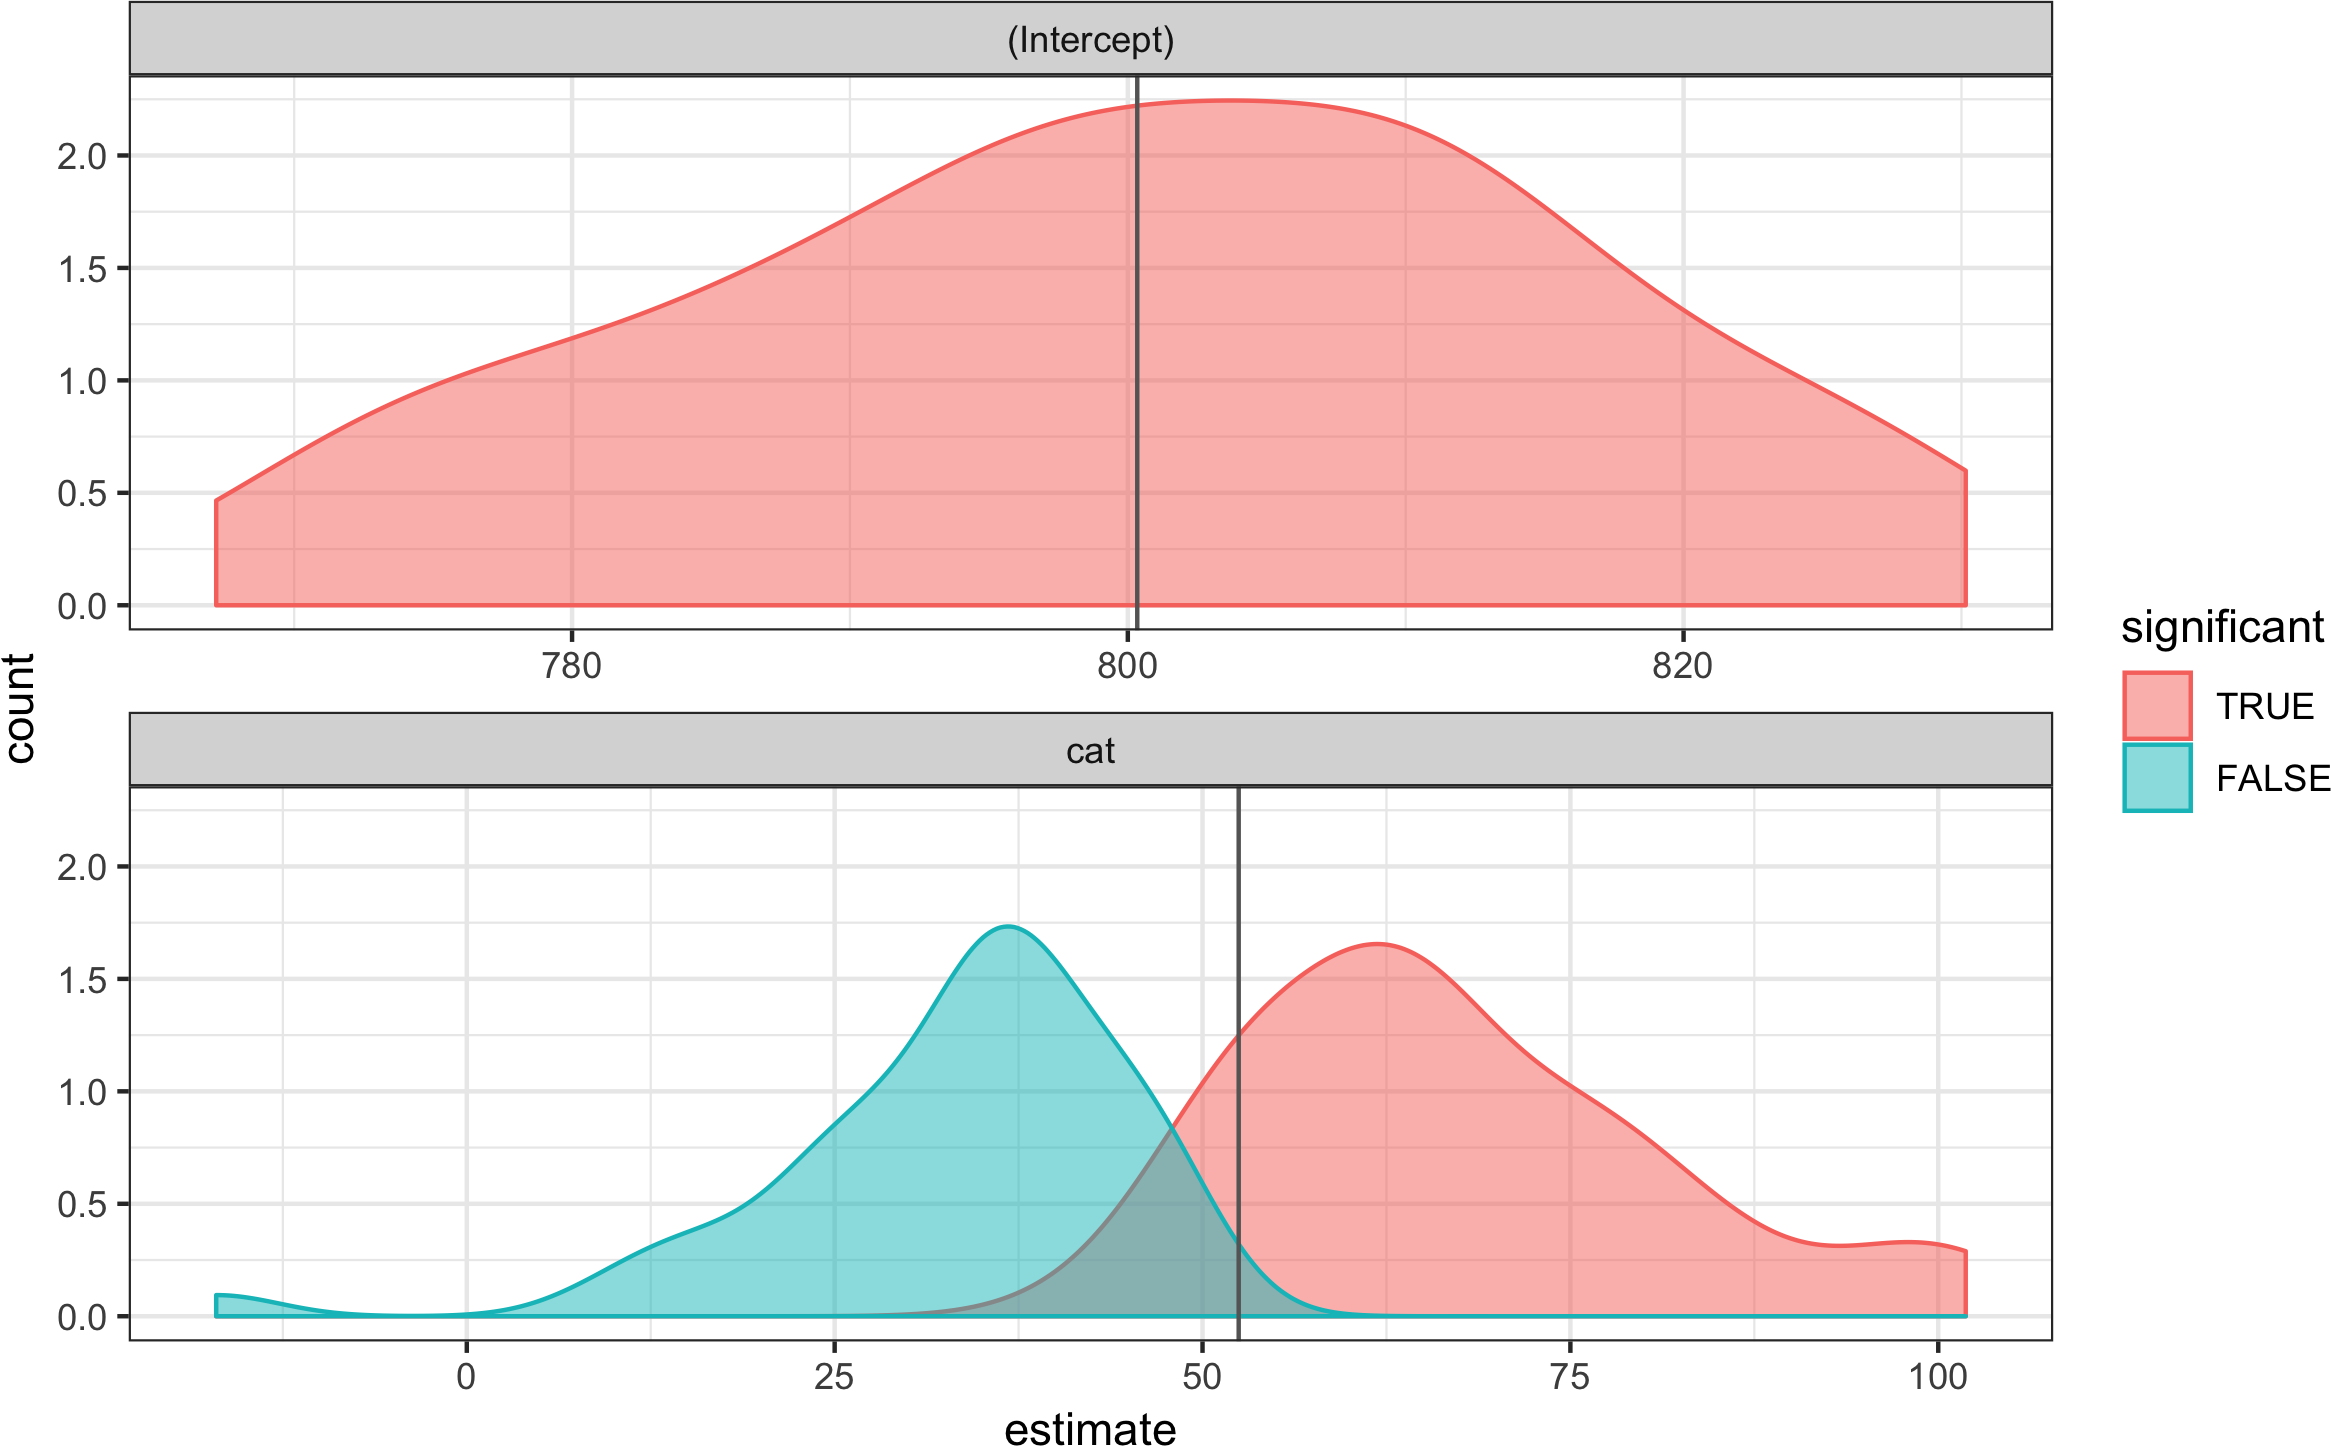
\includegraphics[width=1\linewidth]{images/sim-fixef-plot-1} 

}

\caption{Distribution of fixed effects across 1000 simulations}\label{fig:sim-fixef-plot}
\end{figure}

\begin{figure}

{\centering 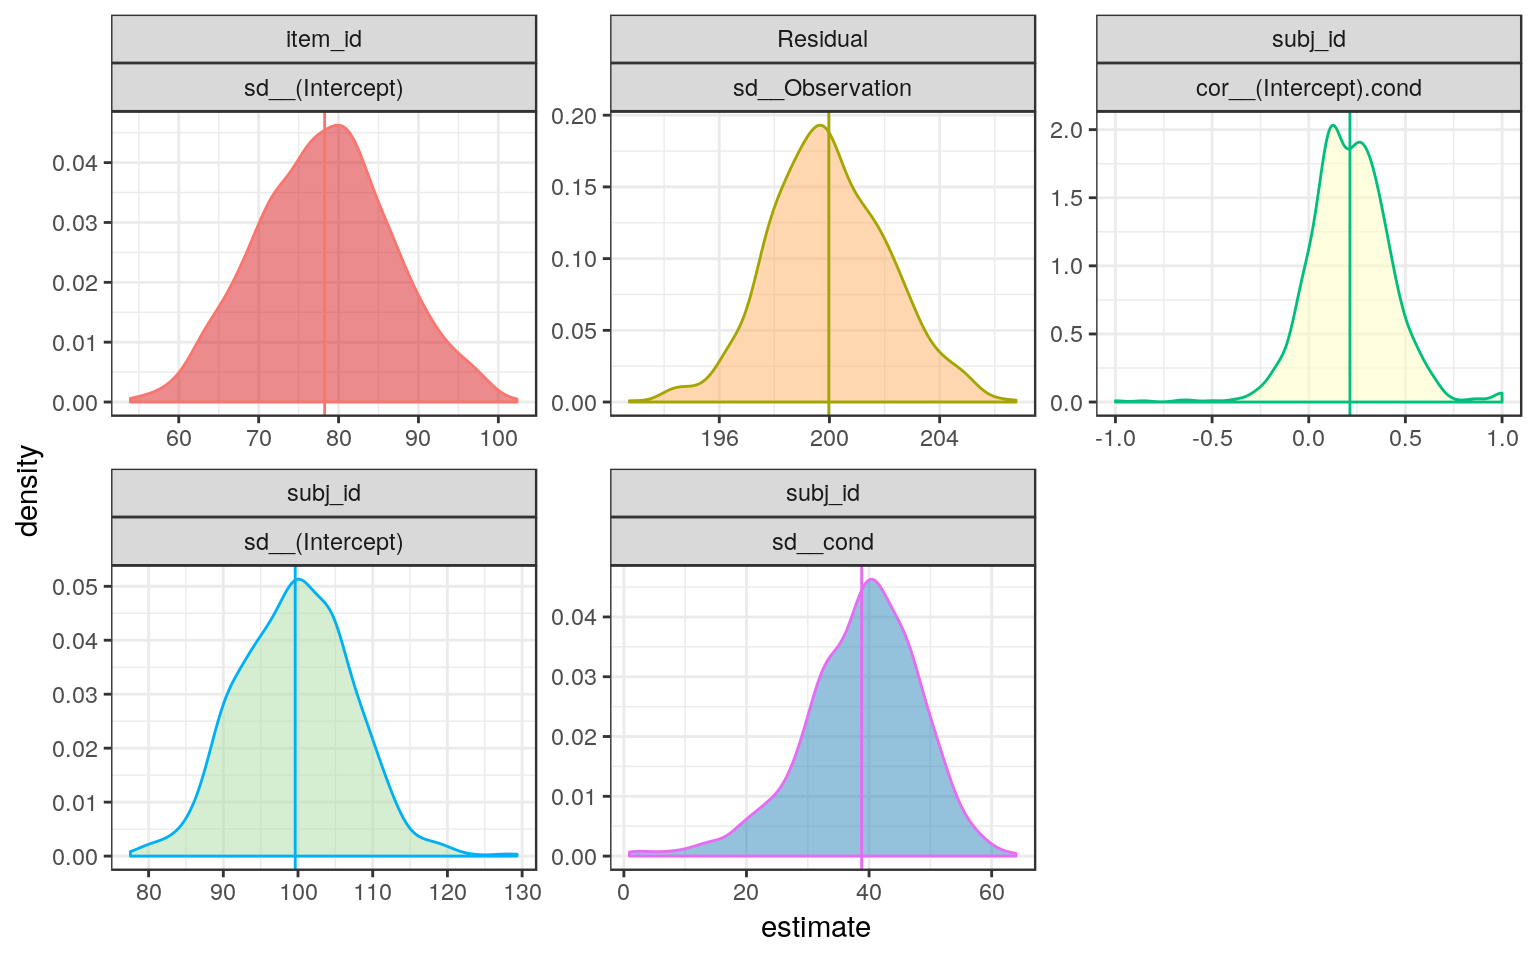
\includegraphics[width=1\linewidth]{images/sim-ranef-plot-1} 

}

\caption{Distribution of random effects across 1000 simulations}\label{fig:sim-ranef-plot}
\end{figure}

\subsection{Comparison to ANOVA}\label{comparison-to-anova}

One way many researchers would normally analyse data like this is by
averaging each subject's reaction times across the ingroup and outgroup
stimuli and compare them using a paired-samples t-test or ANOVA (which
is formally equivalent). Here, we use \texttt{afex::aov\_ez} to analyse
a version of our dataset that is aggregated by subject.

Alternatively, you could aggregate by item, averaging all subjects'
scores for each item.

\begin{Shaded}
\begin{Highlighting}[]
\NormalTok{dat_item <-}\StringTok{  }\NormalTok{dat_sim }\OperatorTok
\StringTok{  }\KeywordTok{group_by}\NormalTok{(item_id, condition, cond) }\OperatorTok
\StringTok{  }\KeywordTok{summarise}\NormalTok{(}\DataTypeTok{RT =} \KeywordTok{mean}\NormalTok{(RT))}

\NormalTok{a_item <-}\StringTok{ }\NormalTok{afex}\OperatorTok{::}\KeywordTok{aov_ez}\NormalTok{(}
  \DataTypeTok{id =} \StringTok{"item_id"}\NormalTok{,}
  \DataTypeTok{dv =} \StringTok{"RT"}\NormalTok{,}
  \DataTypeTok{between =} \StringTok{"condition"}\NormalTok{,}
  \DataTypeTok{data =}\NormalTok{ dat_item}
\NormalTok{)}
\end{Highlighting}
\end{Shaded}

We can create a new power analysis function that simulates data using
our data generating model from \texttt{my\_sim\_data()}, creates these
two aggregated datasets, and analyses them with ANOVAs. Here, we'll just
return the p-values for the effect of interest.

\begin{Shaded}
\begin{Highlighting}[]
\NormalTok{my_anova_power <-}\StringTok{ }\ControlFlowTok{function}\NormalTok{(...) \{}
\NormalTok{  dat_sim <-}\StringTok{ }\KeywordTok{my_sim_data}\NormalTok{(...)}
  
\NormalTok{  dat_subj <-}\StringTok{  }\NormalTok{dat_sim }\OperatorTok
\StringTok{    }\KeywordTok{group_by}\NormalTok{(subj_id, condition, cond) }\OperatorTok
\StringTok{    }\KeywordTok{summarise}\NormalTok{(}\DataTypeTok{RT =} \KeywordTok{mean}\NormalTok{(RT))}
  
\NormalTok{  dat_item <-}\StringTok{  }\NormalTok{dat_sim }\OperatorTok
\StringTok{    }\KeywordTok{group_by}\NormalTok{(item_id, condition, cond) }\OperatorTok
\StringTok{    }\KeywordTok{summarise}\NormalTok{(}\DataTypeTok{RT =} \KeywordTok{mean}\NormalTok{(RT))}

\NormalTok{  a_subj <-}\StringTok{ }\NormalTok{afex}\OperatorTok{::}\KeywordTok{aov_ez}\NormalTok{(}\DataTypeTok{id =} \StringTok{"subj_id"}\NormalTok{,}
                         \DataTypeTok{dv =} \StringTok{"RT"}\NormalTok{,}
                         \DataTypeTok{within =} \StringTok{"condition"}\NormalTok{,}
                         \DataTypeTok{data =}\NormalTok{ dat_subj)}
  \KeywordTok{suppressMessages}\NormalTok{(}
    \CommentTok{# check contrasts message is annoying}
\NormalTok{    a_item <-}\StringTok{ }\NormalTok{afex}\OperatorTok{::}\KeywordTok{aov_ez}\NormalTok{(}
      \DataTypeTok{id =} \StringTok{"item_id"}\NormalTok{,}
      \DataTypeTok{dv =} \StringTok{"RT"}\NormalTok{,}
      \DataTypeTok{between =} \StringTok{"condition"}\NormalTok{,}
      \DataTypeTok{data =}\NormalTok{ dat_item}
\NormalTok{    )}
\NormalTok{  )}
  
  \KeywordTok{list}\NormalTok{(}
    \StringTok{"subj"}\NormalTok{ =}\StringTok{ }\NormalTok{a_subj}\OperatorTok{$}\NormalTok{anova_table}\OperatorTok{$}\StringTok{`}\DataTypeTok{Pr(>F)}\StringTok{`}\NormalTok{,}
    \StringTok{"item"}\NormalTok{ =}\StringTok{ }\NormalTok{a_item}\OperatorTok{$}\NormalTok{anova_table}\OperatorTok{$}\StringTok{`}\DataTypeTok{Pr(>F)}\StringTok{`}
\NormalTok{  )}
\NormalTok{\}}
\end{Highlighting}
\end{Shaded}

Run this function with the default parameters to determine the power
each analysis has to detect an effect of condition of 80 ms.

\begin{Shaded}
\begin{Highlighting}[]
\NormalTok{alpha <-}\StringTok{ }\FloatTok{0.05}

\NormalTok{reps <-}\StringTok{ }\DecValTok{100}
\NormalTok{anova_sims <-}\StringTok{ }\NormalTok{purrr}\OperatorTok{::}\KeywordTok{map_df}\NormalTok{(}\DecValTok{1}\OperatorTok{:}\NormalTok{reps, }\OperatorTok{~}\KeywordTok{my_anova_power}\NormalTok{())}

\NormalTok{power_subj <-}\StringTok{ }\KeywordTok{mean}\NormalTok{(anova_sims}\OperatorTok{$}\NormalTok{subj }\OperatorTok{<}\StringTok{ }\NormalTok{alpha)}
\NormalTok{power_item <-}\StringTok{ }\KeywordTok{mean}\NormalTok{(anova_sims}\OperatorTok{$}\NormalTok{item }\OperatorTok{<}\StringTok{ }\NormalTok{alpha)}
\end{Highlighting}
\end{Shaded}

The by-subjects ANOVA has power of 1, while the by-items ANOVA has power
of 0.89. This isn't simply a consequence of within versus between design
or the number of subjects versus items, but rather a consequence of the
inflected false positive rate of some aggregated analyses.

Set the effect of condition to 0 to calculate the false positive rate.
This is the probability of concluding there is an effect when there is
no actual effect in your population.

\begin{Shaded}
\begin{Highlighting}[]
\NormalTok{reps <-}\StringTok{ }\DecValTok{100}
\NormalTok{anova_fp <-}\StringTok{ }\NormalTok{purrr}\OperatorTok{::}\KeywordTok{map_df}\NormalTok{(}\DecValTok{1}\OperatorTok{:}\NormalTok{reps, }\OperatorTok{~}\KeywordTok{my_anova_power}\NormalTok{(}\DataTypeTok{b1 =} \DecValTok{0}\NormalTok{))}

\NormalTok{false_pos_subj <-}\StringTok{ }\KeywordTok{mean}\NormalTok{(anova_fp}\OperatorTok{$}\NormalTok{subj }\OperatorTok{<}\StringTok{ }\NormalTok{alpha)}
\NormalTok{false_pos_item <-}\StringTok{ }\KeywordTok{mean}\NormalTok{(anova_fp}\OperatorTok{$}\NormalTok{item }\OperatorTok{<}\StringTok{ }\NormalTok{alpha)}
\end{Highlighting}
\end{Shaded}

Ideally, your false positive rate will be equal to alpha, which we set
here at 0.05. You can see that the by-subject aggregated analysis has a
massively inflated false positive rate of 0.51. This is not a mistake,
but a consequence of averaging items and analysing a between-item
factor.

\subsection{Conclusion}\label{conclusion}

In this tutorial, we have introduced the main concepts needed to get
started with mixed effect models. Through data simulation, you can
develop your understanding and perform power calculations to guide your
sample size plans. We have also demonstrated through simulation the
dangers of aggregating data over a unit of analysis. The R code in this
tutorial is supplemented by a
\href{http://shiny.psy.gla.ac.uk/lmem/}{Shiny app} that will allow you
to change parameters and inspect the results of LMEM and ANOVA analyses,
as well as calculate power and false positives for these analyses.

\subsubsection{Glossary}\label{glossary}

\begin{longtable}[]{@{}ll@{}}
\toprule
Term & Definition\tabularnewline
\midrule
\endhead
by-subjects analysis (\(F_1\)) & def\tabularnewline
by-items analysis (\(F_2\)) & def\tabularnewline
crossed random factors & def\tabularnewline
data-generating process & def\tabularnewline
deflection & def\tabularnewline
fixed effect & def\tabularnewline
intercept/grand mean & def\tabularnewline
random effect & def\tabularnewline
random intercept & def\tabularnewline
random slope & def\tabularnewline
slope & def\tabularnewline
\bottomrule
\end{longtable}

\newpage

\section{References}\label{references}

\begingroup
\setlength{\parindent}{-0.5in} \setlength{\leftskip}{0.5in}

\hypertarget{refs}{}
\hypertarget{ref-baayen_davidson_bates_2008}{}
Baayen, R. H., Davidson, D. J., \& Bates, D. M. (2008). Mixed-effects
modeling with crossed random effects for subjects and items.
\emph{Journal of Memory and Language}, \emph{59}, 390--412.

\hypertarget{ref-barr_2018}{}
Barr, D. J. (2018). Generalizing over encounters: Statistical and
theoretical considerations. In S.-A. Rueschemeyer \& M. G. Gaskell
(Eds.), \emph{Oxford handbook of psycholinguistics}. Oxford University
Press.

\hypertarget{ref-barr_et_al_2013}{}
Barr, D. J., Levy, R., Scheepers, C., \& Tily, H. J. (2013). Random
effects structure for confirmatory hypothesis testing: Keep it maximal.
\emph{Journal of Memory and Language}, \emph{68}(3), 255--278.

\hypertarget{ref-R-lme4}{}
Bates, D., Mächler, M., Bolker, B., \& Walker, S. (2015). Fitting linear
mixed-effects models using lme4. \emph{Journal of Statistical Software},
\emph{67}(1), 1--48.
doi:\href{https://doi.org/10.18637/jss.v067.i01}{10.18637/jss.v067.i01}

\hypertarget{ref-bedny_aguirre_thompson-schill_2007}{}
Bedny, M., Aguirre, G. K., \& Thompson-Schill, S. L. (2007). Item
analysis in functional magnetic resonance imaging. \emph{Neuroimage},
\emph{35}(3), 1093--1102.

\hypertarget{ref-clark_1973}{}
Clark, H. H. (1973). The language-as-fixed-effect fallacy: A critique of
language statistics in psychological research. \emph{Journal of Verbal
Learning and Verbal Behavior}, \emph{12}, 335--359.

\hypertarget{ref-coleman_1964}{}
Coleman, E. B. (1964). Generalizing to a language population.
\emph{Psychological Reports}, \emph{14}, 219--226.

\hypertarget{ref-R-faux}{}
DeBruine, L. (2019). \emph{Faux (beta) (version v0.0.0.9011-beta)}.
Zenodo.
doi:\href{https://doi.org/10.5281/zenodo.2669587}{10.5281/zenodo.2669587}

\hypertarget{ref-forster_dickinson_1976}{}
Forster, K., \& Dickinson, R. (1976). More on the
language-as-fixed-effect fallacy: Monte carlo estimates of error rates
for \(F_1\),\(F_2\),\(F'\), and min \(F'\). \emph{Journal of Verbal
Learning and Verbal Behavior}, \emph{15}, 135--142.

\hypertarget{ref-judd_westfall_kenny_2012}{}
Judd, C. M., Westfall, J., \& Kenny, D. A. (2012). Treating stimuli as a
random factor in social psychology: A new and comprehensive solution to
a pervasive but largely ignored problem. \emph{Journal of Personality
and Social Psychology}, \emph{103}, 54.

\hypertarget{ref-TOSTtutorial}{}
Lakens, D., Scheel, A. M., \& Isager, P. M. (2018). Equivalence testing
for psychological research: A tutorial. \emph{Advances in Methods and
Practices in Psychological Science}, \emph{1}(2), 259--269.
doi:\href{https://doi.org/10.1177/2515245918770963}{10.1177/2515245918770963}

\hypertarget{ref-locker_hoffman_bovaird_2007}{}
Locker, L., Hoffman, L., \& Bovaird, J. (2007). On the use of multilevel
modeling as an alternative to items analysis in psycholinguistic
research. \emph{Behavior Research Methods}, \emph{39}, 723--730.

\hypertarget{ref-R-base}{}
R Core Team. (2018). \emph{R: A language and environment for statistical
computing}. Vienna, Austria: R Foundation for Statistical Computing.
Retrieved from \url{https://www.R-project.org/}

\hypertarget{ref-westfall_yarkoni_2016}{}
Westfall, J., Nichols, T. E., \& Yarkoni, T. (2016). Fixing the
stimulus-as-fixed-effect fallacy in task fMRI. \emph{Wellcome Open
Research}, \emph{1}.

\endgroup


\end{document}
